\documentclass[t, 11pt]{beamer}
\usepackage{mathtools}
\usepackage{pdfpages}
\usepackage{graphicx}
\usepackage{tikz}
\usepackage{multimedia}
\usepackage{transparent}
\usetikzlibrary{calc}

%%%%%%%%%%%%%%%%%%%%%%%%%%%%%%%%%%%%%%%%%%%%%%%%%%%%%%%%%%%%
% Useful things

% list
%% \begin{itemize}
%% \item List a
%% \item List b
%% \end{itemize}

% image
%% \begin{center}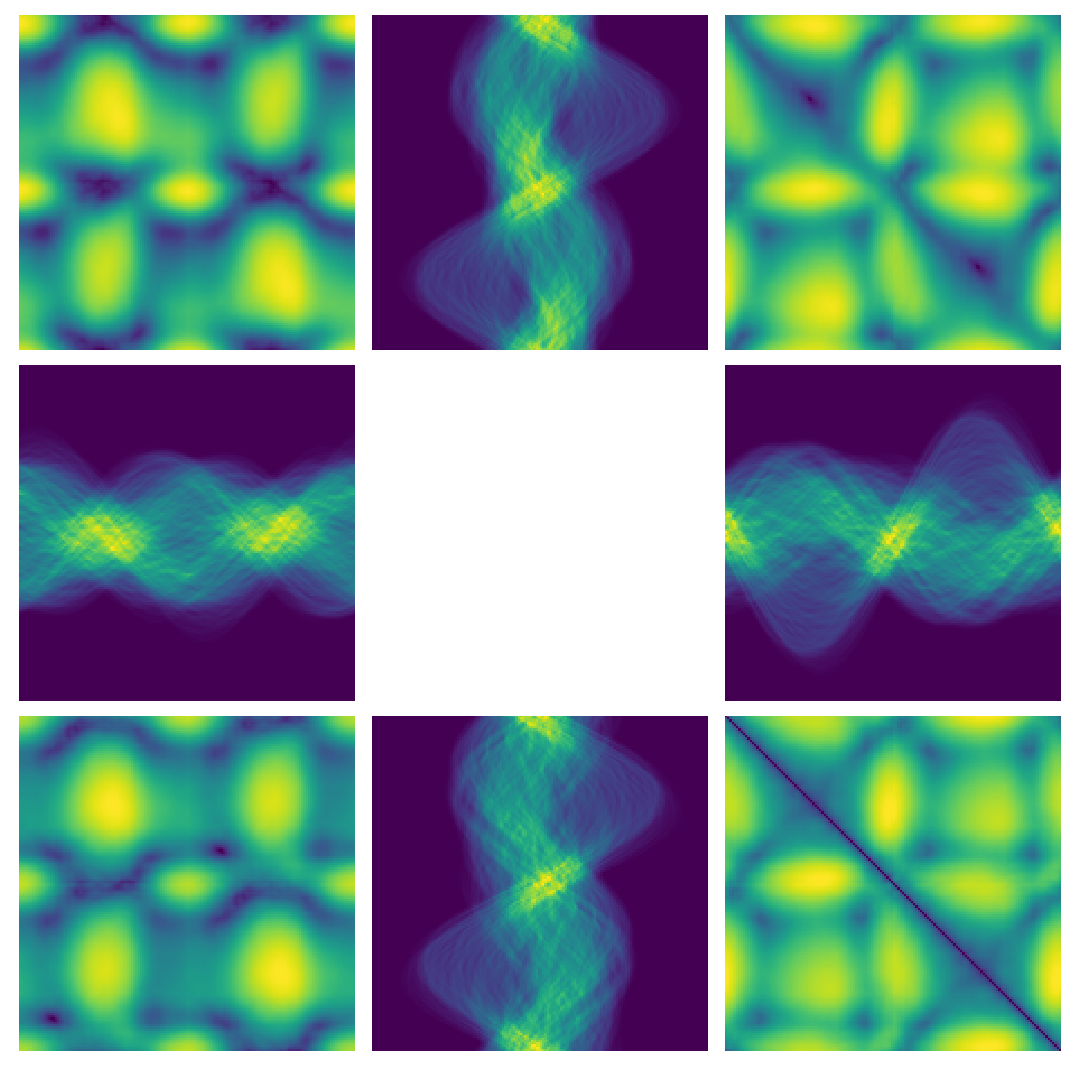
\includegraphics[width=0.45\textwidth]{images/Sinogram_3_comp.png}
%% \end{center}

% absolute position
%% \placetextbox[north west]{0.37}{0.33}{\setlength{\fboxsep}{0pt}\setlength{\fboxrule}{0.5pt}\fbox{absolute position1}}
%% \placetextbox[north west]{0.77}{0.33}{\setlength{\fboxsep}{0pt}\setlength{\fboxrule}{0.5pt}\fbox{absolute postion 2}}

% movie
%% \placetextbox[north west]{0.083}{0.30}{\movie[width=3.5cm,height=2cm,poster, externalviewer, loop]{\includegraphics[width=3.5cm]{movie_still.png}}{movie.webm}}
%%%%%%%%%%%%%%%%%%%%%%%%%%%%%%%%%%%%%%%%%%%%%%%%%%%%%%%%%%%%

%%%%%%%%%%%%%%%%%%%%%%%%%%%%%%%%%%%%%%%%%%%%%%%%%%%%%%%%%%%%
% absolute positioning of typeset material    
%%%%%%%%%%%%%%%%%%%%%%%%%%%%%%%%%%%%%%%%%%%%%%%%%%%%%%%%%%%%
\newcommand{\placetextbox}[4][center]{%
  % [#1]: box anchor: center (default) | 
  %                 south west | west | north west | north |
  %                 north east | east | south east | south | 
  %                 mid west | mid | mid east |
  %                 base west | base | base east 
  % #2: horizontal position (fraction of page width)
  % #3: vertical position (fraction of page height)
  % #4: content
  %
  \tikz[remember picture,overlay,x=\paperwidth,y=\paperheight]{%
    \node[anchor=#1,inner sep=0pt]
    at ($(current page.south west)+(#2,#3)$) {#4};
  }%
}
%%%%%%%%%%%%%%%%%%%%%%%%%%%%%%%%%%%%%%%%%%%%%%%%%%%%%%%%%%%%

% \usetheme{Madrid}
\usetheme{Berlin}

\def\liketitle#1{%
{\usebeamerfont{frametitle}\usebeamercolor[fg]{structure}%
\begin{flushleft}%
\vspace{-\baselineskip}% Cometic correction for space introduced by flushleft
#1\par
\end{flushleft}%
\vspace{-\baselineskip}% Cosmetic correction for space introduced by flushleft
}%
\vspace{0.75\baselineskip}%
}

\date{March 23rd, 2020}
\author{Donovan Webb}
\institute{eBIC/University of Bath}
\titlegraphic{
\includegraphics[width=3cm]{images/Diamond.png}}
\title{Classification and Reconstruction from Single Lines}

\AtBeginSection[]{
  \begin{frame}
  \vfill
  \centering
  \begin{beamercolorbox}[sep=8pt,center,shadow=false,rounded=false]{title}
    \usebeamerfont{title}\insertsectionhead\par%
  \end{beamercolorbox}
  \vfill
  \end{frame}
}

\begin{document}

\setbeamertemplate{navigation symbols}{}
\begin{frame}[plain]
  \maketitle
\end{frame}
\addtocounter{framenumber}{-1} % Don't count title slide

\begin{frame}{Table of Contents}
  \tableofcontents[sectionstyle=show/show, hideallsubsections]
\end{frame}


\section{Single Lines}
\subsection{Sinograms}

\begin{frame}[fragile]{The Radon Transform}
 \only<1>{\begin{center}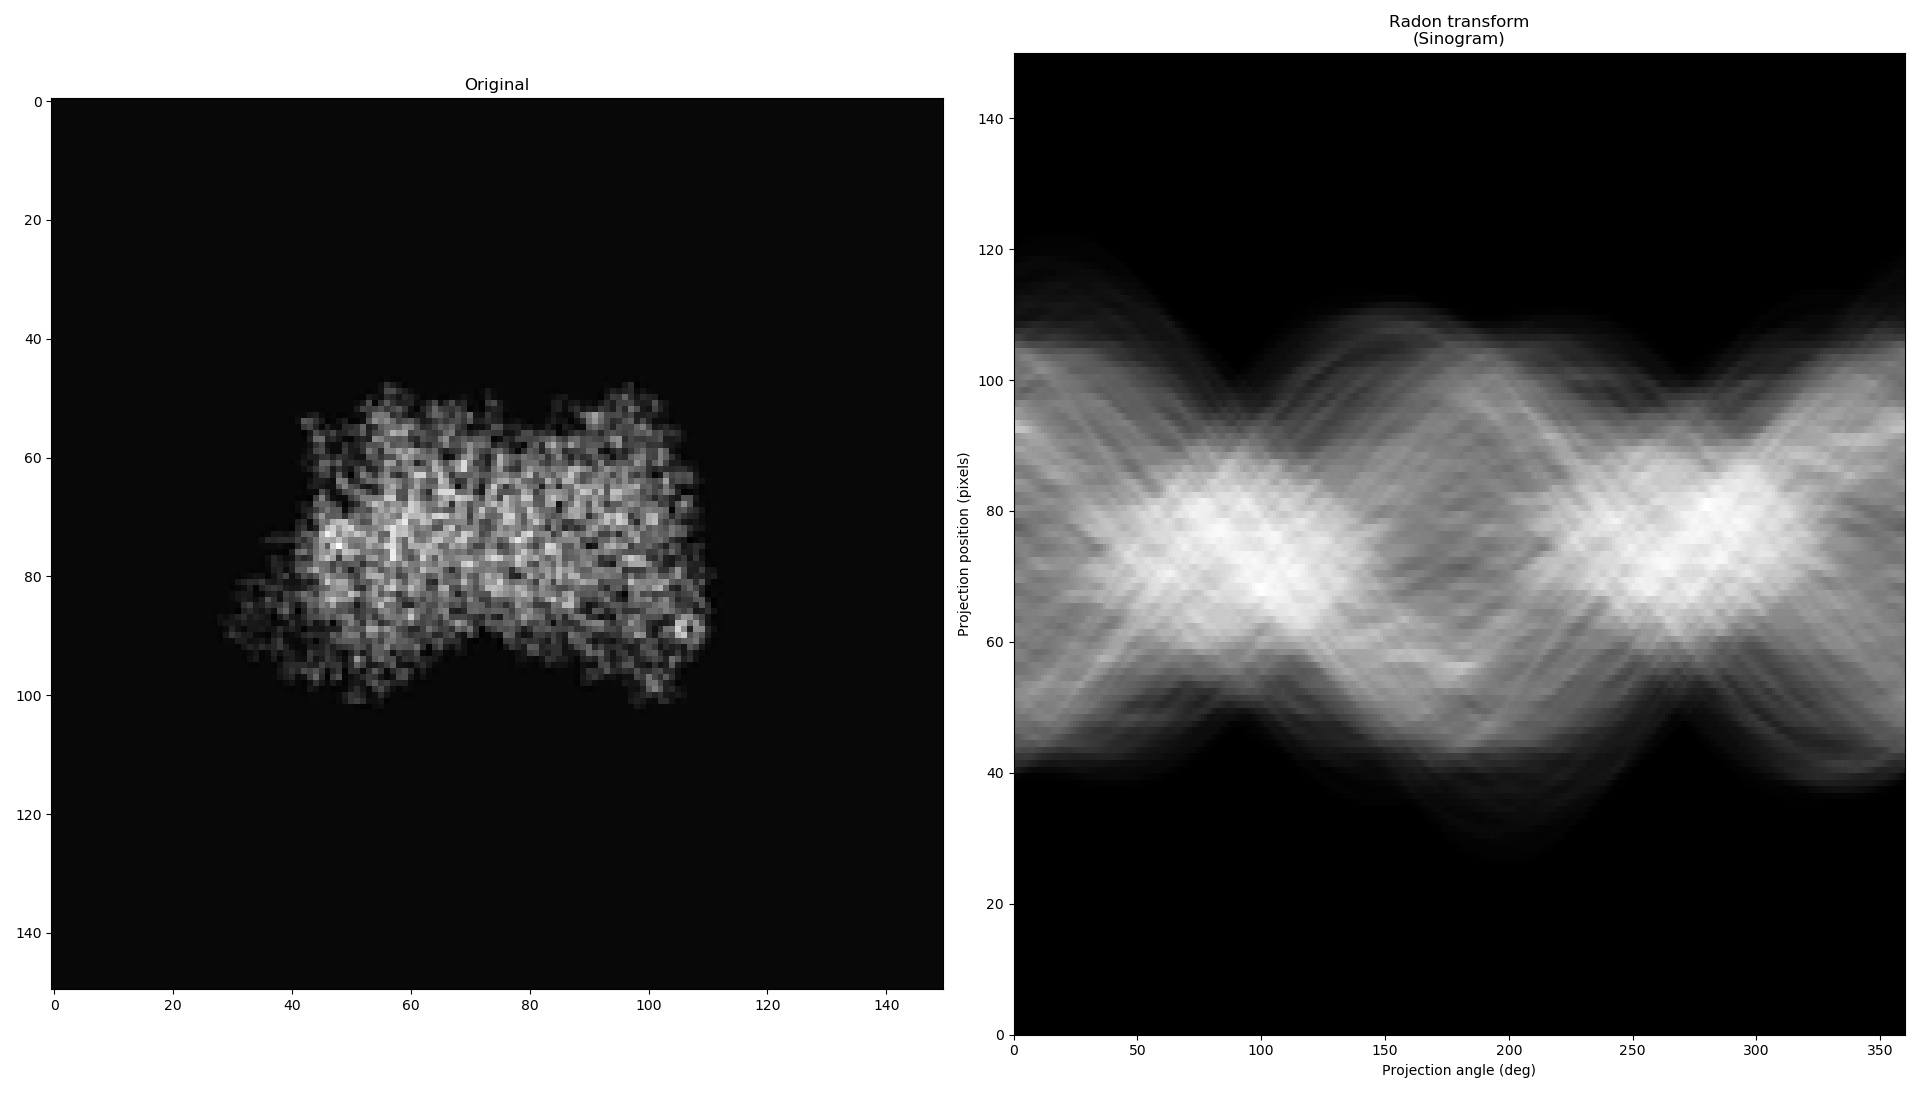
\includegraphics[width=0.65\textwidth]{images/Sinogram_Proj1.png}
    \end{center}}
\vspace{-1em}
 \only<2>{\begin{center}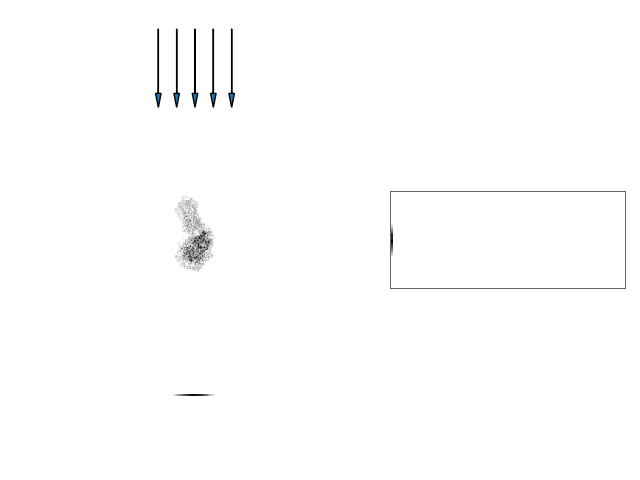
\includegraphics[width=0.85\textwidth]{images/sino_ani/sino_make_fr1.png}
    \end{center}}
 \only<3>{\begin{center}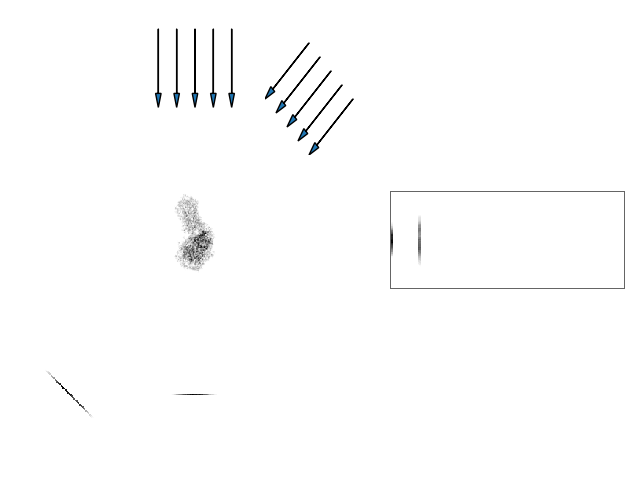
\includegraphics[width=0.85\textwidth]{images/sino_ani/sino_make_fr2.png}
    \end{center}}
 \only<4>{\begin{center}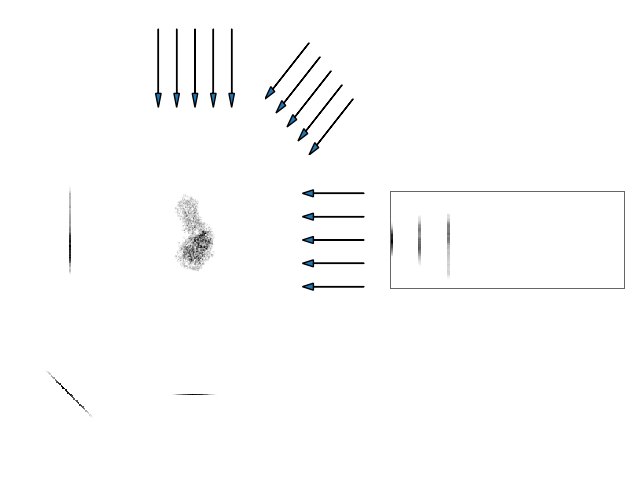
\includegraphics[width=0.85\textwidth]{images/sino_ani/sino_make_fr3.png}
    \end{center}}
 \only<5>{\begin{center}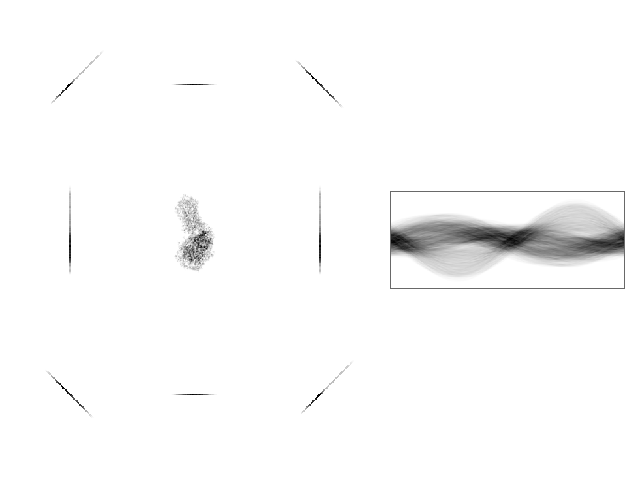
\includegraphics[width=0.85\textwidth]{images/sino_ani/sino_make_fr4.png}
    \end{center}}

\end{frame}

\begin{frame}[fragile]{Common Lines}

  \textbf{Two projections of the same 3D volume share at least one common line in the Radon transform}
 \begin{center}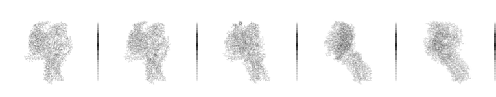
\includegraphics[width=0.85\textwidth]{images/common_line.png}
    \end{center}
 \begin{center}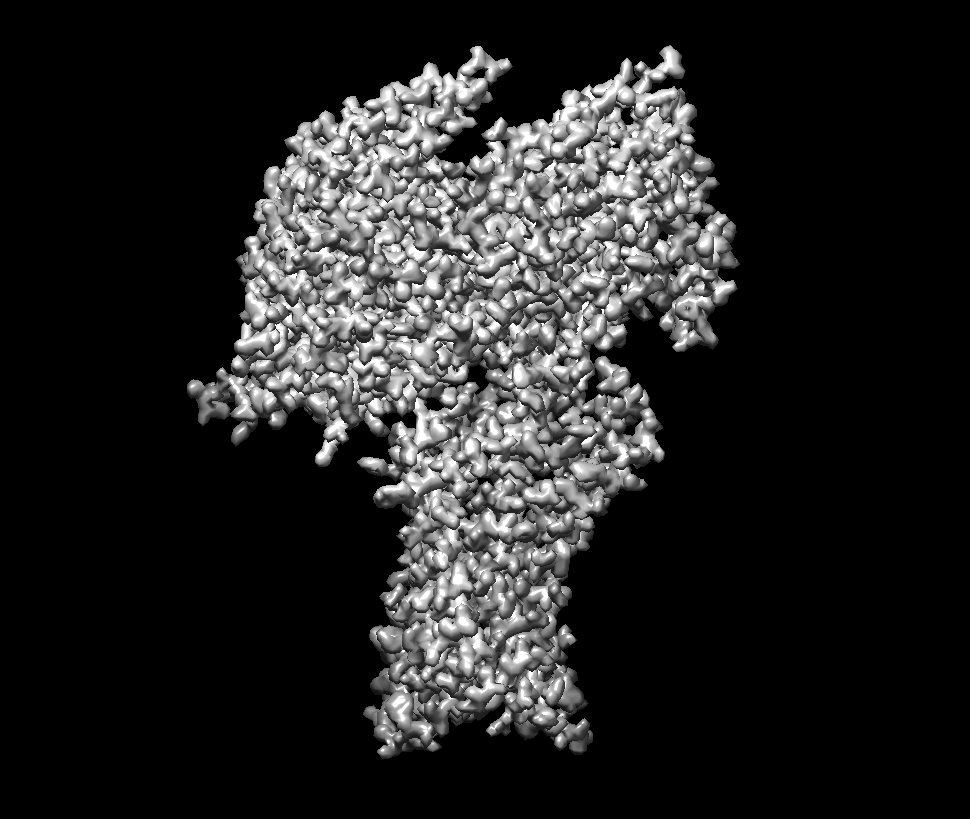
\includegraphics[width=0.35\textwidth]{images/3D_model.png}
    \end{center}

\end{frame}

\begin{frame}[fragile]{Comparing single lines}
  Show different methods.
  Cross correlation,
  show single line as signal
  Problems! translation, noise, ctf...
\end{frame}

\begin{frame}[fragile]{Detour! Angular recovery from 3 Common lines}
  \textit{\tiny{Angular Reconstitution: A Posteriori Assignment of Projection Directions for 3d Reconstruction. Van Heel 1987}}
  \textbf{Common line gives axis of rotation}
  Three common lines gives 2 unique solutions for 3D orientation (One mirror of other)
  \begin{center}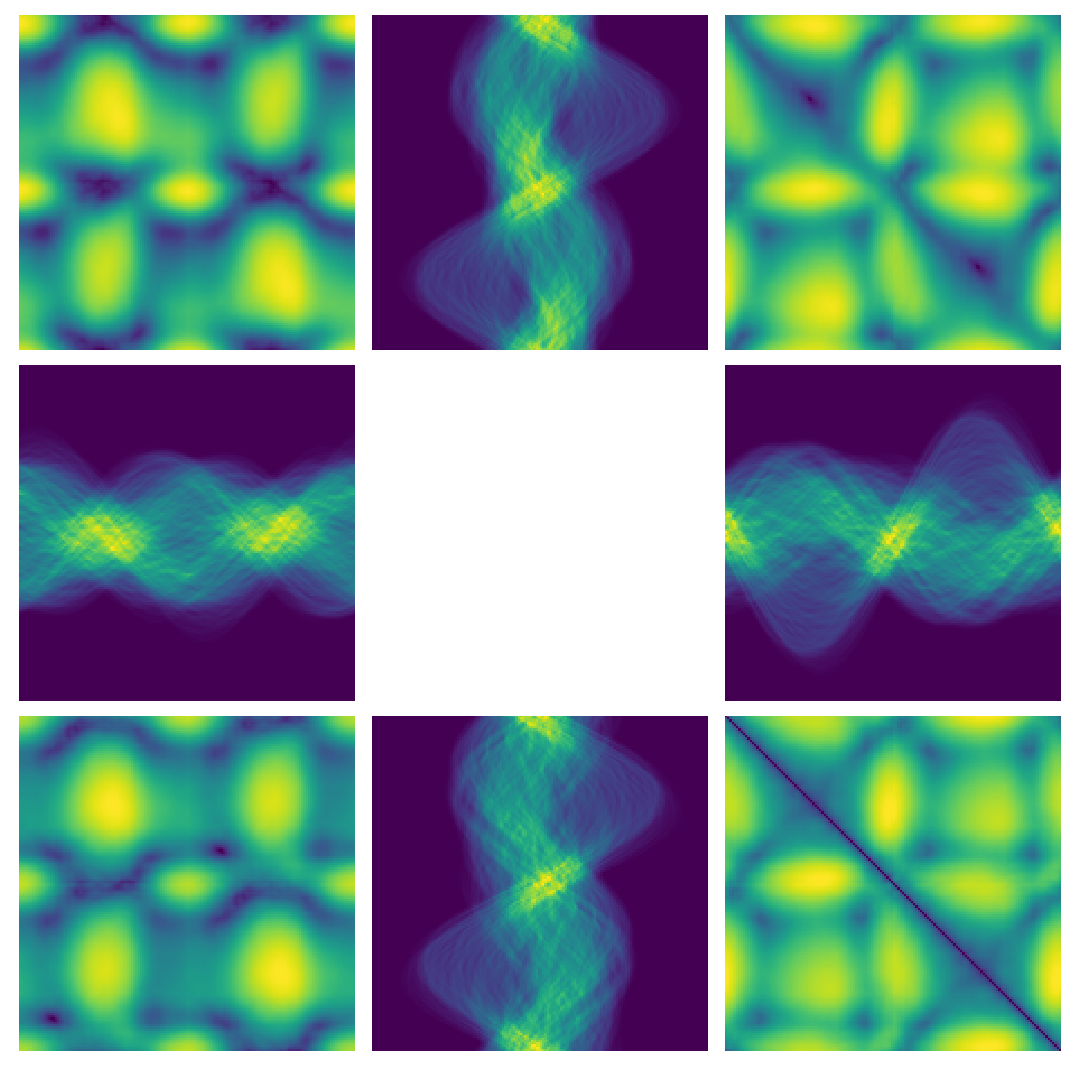
\includegraphics[width=0.45\textwidth]{images/Sinogram_3_comp.png}
    \end{center}
\end{frame}


\begin{frame}[fragile]{Detour2! crYOLO}
  Particle picking improvements mean no longer have to rely on 2D classes to get sinograms from...
  Good centering, only particles being picked.
  Extensive use at eBIC will touch at the end...
\end{frame}


\section{Finding Common Lines}
\subsection*{Nearest Neighbour}

\begin{frame}[fragile]{Raw single lines}
  Procedure for finding common lines. Get euclidian distances. Smallest is most similar
\end{frame}

\begin{frame}[fragile]{Dimensional Reduction}
  Dimensional reduction can be used to lower influence of noise and try to find common features of data.
  Manifold learning found to improve accuracy of common lines being chosen although more computationally expensive.
  Plot 2D pca of sinogram
  and non-linear Iso map or lle
\end{frame}

\begin{frame}[fragile]{Comparison between linear and non-linear dimensions}
  Graph of how lin vs non-lin change for different noise levels and different number of components
\end{frame}

\begin{frame}[fragile]{Bonus slide: NN architecture for comparing single lines}
  Could we use NN to find filters? Number of attempts but nothing stable as yet.
  Probably leave out as unsuccesful and long to explain - could do a passing mention
\end{frame}

\section{Reconstruction}
\subsection*{Too many Lines}
\begin{frame}[fragile]{Voting}
  Take all lines pairs under distance X
  This gives multiple possible axis between the same two projections. Weight these according to distance and number of times they appear.
  For each common line between two sinograms get more than 1 match so... vote which is best!
\end{frame}

\begin{frame}[fragile]{Over determined system}
  3 lines is all good for getting angular information back c.f. prev slide.
  any more than 3 and we can get contradicting equations - system is overdetermined. we have N\^2 linear equations and only 6N variables (do proper maths)
  Machine learning 3! how to fit. Least squares optimization not good as we have large number of misidentified lines and nonconvex! we also need to get proper rotation matrices at the end. This constraint leads to collapse to trivial solution 000. Need other approach.
\end{frame}

\begin{frame}[fragile]{Eigenvector Relaxation}
  \small
  \textbf{Aim: Given all common lines $c$ for projections $P$, assign Rotation matrices $R$ for each $P$ to give greatest consensus volume.} \\
  Image of Radon with angles. Image of FT with angles.\\
  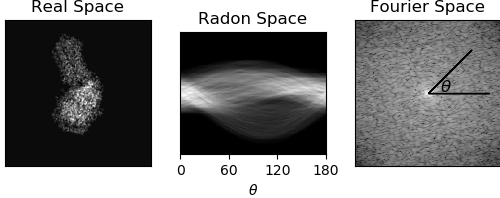
\includegraphics[width=0.35\textwidth]{images/radon_ft.png}
\vspace{-3.7em}
  \hspace{3em}\tiny{$$\hspace{15em}cij~=~(cos(\theta_{ij}),sin(\theta_{ij}),0),~cji~=~(cos(\theta_{ji}),sin(\theta_{ji}),0)~\quad~(1)$$}

  \small
  $$max\sum_{i\ne j} R_ic_{ij} \cdot R_jc_{ji} \quad (2)$$
  Maths*! Make large $(2N \times 2N)$ symmetric matrix $S$. Can recover $R$ for each $P$ from top 3 eigenvectors of $S$ that maximise (2)! \\
  Image of eigenvalue histogram
  % Explain in simple-ish terms Singer Shkolnisky method for finding Rotation matrices for each projection.
  % Made in python! Using common lines in sinograms instead of in fourier. Maybe explain relationship between two. 
  % Show their results of how no. of correct common lines affect final result.
  

  \textit{\tiny{*Three Dimensional Structure Determination from Common Lines in Cryo-EM by Eigenvectors and Semidefinite Programming. A.Singer and Y.Shkolnisky}}
\end{frame}

\begin{frame}[fragile]{Models!}
  Lots of models!
\end{frame}

\begin{frame}[fragile]{Computational efficiency}
  only calculating 95\% of correct lines make others random. 6x speed increase. Parrallelisation needed!
  Show that adding random lines does not affect recon too much..
\end{frame}

\begin{frame}[fragile]{Priming matrix with tilt data! - Not done yet}
  With tilt data we know the tilt axis (and angle but this is not important)
  Can calculate what common single line would be for this data would be. can input straight into matrix
\end{frame}


\section{Clustering - Not done yet}
\subsection{}
\begin{frame}{Can heterogenaity be sorted by looking at common lines?}
 % Columns/transparancy and slide animations
\begin{columns}
\begin{column}{.5\textwidth}
\liketitle{\only<2>{\transparent{0.4}}~~A}
  \begin{itemize}
  \only<2>{\transparent{0.4}}
    \vspace{1.2em}
    \item[\only<2>{\transparent{0.4}}{\textbullet}] Lorem Ipsum
    \vspace{1em}
    \item[\only<2>{\transparent{0.4}}{\textbullet}] Dolor est
    \vspace{1em}
    \item[\only<2>{\transparent{0.4}}{\textbullet}] Example incoming
    \vspace{1em}
    \item[\only<2>{\transparent{0.4}}{\textbullet}] Example arrived
  \end{itemize} 
\end{column}
\begin{column}{.5\textwidth}
\liketitle{\only<1>{\transparent{0.4}}~B}
  \begin{itemize}
\only<1>{\transparent{0.4}}
    \vspace{0.7em}
    \item[\only<1>{\transparent{0.4}}{\textbullet}] Sometimes its hard to make up random content
    \vspace{0.7em}
    \item[\only<1>{\transparent{0.4}}{\textbullet}] Othertimes not
    \vspace{0.7em}
    \item[\only<1>{\transparent{0.4}}{\textbullet}] Filler words
    \vspace{0.7em}
    \item[\only<1>{\transparent{0.4}}{\textbullet}] And filler phrases that are ever so slightly longer
  \end{itemize} 
\end{column}
\end{columns}
\end{frame}

\end{document}
